\hypertarget{_c_i2_c_8cpp}{\section{Référence du fichier /home/jam/\+Bureau/\+C++/\+Classes/\+C\+I2\+C/\+C\+I2\+C.cpp}
\label{_c_i2_c_8cpp}\index{/home/jam/\+Bureau/\+C++/\+Classes/\+C\+I2\+C/\+C\+I2\+C.\+cpp@{/home/jam/\+Bureau/\+C++/\+Classes/\+C\+I2\+C/\+C\+I2\+C.\+cpp}}
}


Contient la définition de la classe \hyperlink{class_c_i2_c}{C\+I2\+C}.  


{\ttfamily \#include \char`\"{}C\+I2\+C.\+h\char`\"{}}\\*
Graphe des dépendances par inclusion de C\+I2\+C.\+cpp\+:\nopagebreak
\begin{figure}[H]
\begin{center}
\leavevmode
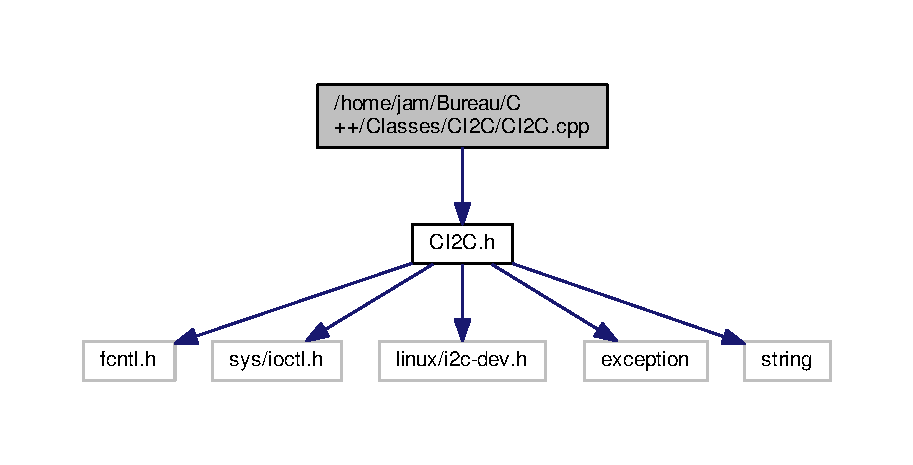
\includegraphics[width=350pt]{_c_i2_c_8cpp__incl}
\end{center}
\end{figure}


\subsection{Description détaillée}
Contient la définition de la classe \hyperlink{class_c_i2_c}{C\+I2\+C}. 



Définition dans le fichier \hyperlink{_c_i2_c_8cpp_source}{C\+I2\+C.\+cpp}.

